\documentclass[pdf]{beamer}

\mode<presentation> {
  \usetheme{Warsaw}
  \setbeamercovered{transparent}
}
\title{Funciones de distribucion de probabilidad}
\author{Marco Antonio Montero Chavarria}
\usepackage{graphicx}
\usepackage{amsmath}
\usepackage[spanish]{babel}
\usepackage[utf8]{inputenc}
\usepackage{babelbib}
\usepackage[T1]{fontenc}
\usepackage{color}
\usepackage{framed}
\usepackage{hyperref}
\usepackage{mathtools}
\usepackage{listings}
\usepackage{newtxmath,newtxtext}
%************************************************
\begin{document}
%%diapositiva para el título
\begin{frame}
 \titlepage
\end{frame}

%%diapositiva normal

\begin{frame}{El problema}
Emular el comportamiento de un sistema de comunicación inalámbrico.
\begin{center}
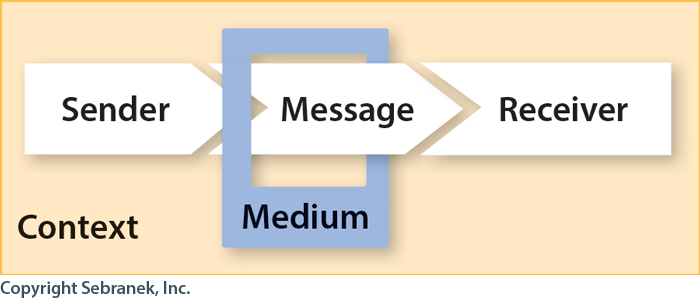
\includegraphics[height=0.5\textheight]{CommunicationSituation.png}
\end{center}
\end{frame}
%********************************************
\begin{frame}{El problema}
Emular el comportamiento de un sistema de comunicación inalámbrico.
\begin{center}
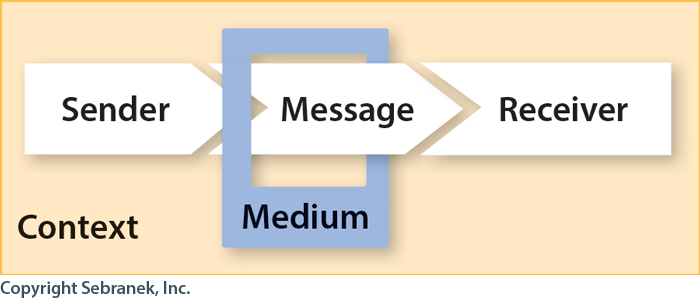
\includegraphics[height=0.5\textheight]{CommunicationSituation.png}
\end{center}
\end{frame}
%********************************************
\begin{frame}{El canal}
El canal o medio es el aire por lo tanto posee ruido.
El ruido es aleatorio. 
\begin{itemize}
\item Ruido Gaussiano
\item Ruido Rayleigh
\end{itemize}
\begin{center}
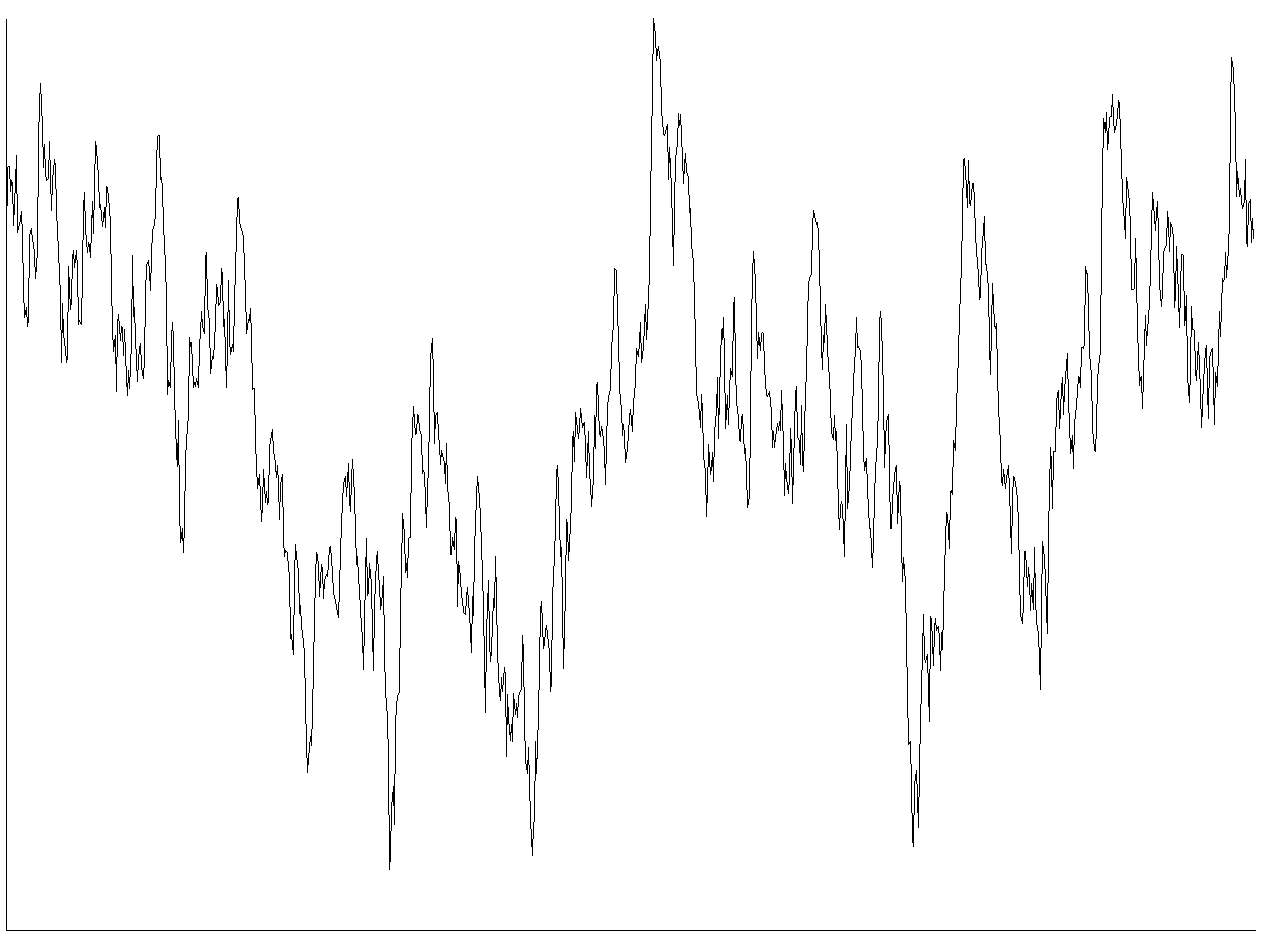
\includegraphics[height=0.4\textheight]{noise.png}
\end{center}
\end{frame}
%********************************************
\begin{frame}{Algoritmo Box-Muller variación polar Marsaglia}
Permite pasar de una distribución uniforme a una distribución gaussiana.
Requiere:
\begin{itemize}
\item Tener 2 variables uniformemente distribuidas entre [-1,1] U1 y U2 que sean independientes.
\end{itemize}
\end{frame}
%********************************************
\begin{frame}{Algoritmo Box-Muller variación polar Marsaglia}
Permite pasar de una distribución uniforme a una distribución gaussiana.
Requiere:
\begin{itemize}
\item Tener 2 variables uniformemente distribuidas entre [-1,1] U1 y U2 que sean independientes.
\end{itemize}
\end{frame}
%********************************************
\begin{frame}{Algoritmo Box-Muller variación polar Marsaglia}
\begin{itemize}
\item Transforma U1 y U2 en Z1 y Z2 que son 2 variables normalmente distribuidas independientes.(con $\mu=0$ y $\sigma = 1$).\\
\item $Z1 = U1* \sqrt{\frac{-2 * \ln w}{w}}$ donde $w = U1*U1 +U2*U2$
\end{itemize}
\end{frame}
%********************************************
\begin{frame}{Algoritmo Box-Muller variación polar Marsaglia}
\begin{itemize}
\item Transforma U1 y U2 en Z1 y Z2 que son 2 variables normalmente distribuidas independientes.(con $\mu=0$ y $\sigma = 1$).\\
\item $Z1 = U1* \sqrt{\frac{-2 * \ln w}{w}}$ donde $w = U1*U1 +U2*U2$
\end{itemize}
\end{frame}
%********************************************
\begin{frame}{Algoritmo Box-Muller variación polar Marsaglia}
Por último:
\begin{itemize}
\item Luego se crea la variable aleateoria $ X= Z * \sigma + \mu $. 
\end{itemize}
Z debe cambiar entre Z1 y Z2.

\end{frame}
%********************************************
\begin{frame}{Algoritmo Box-Muller variación para Rayeligh}
Otra propiedad del método es que el radio R esta distribuido Rayleigh.
\begin{itemize}
\item $X = \sigma \sqrt{-2*\ln U}$. Con U uniformemente distribuida en [0,1]
\end{itemize}
\end{frame}
%********************************************
\begin{frame}{Solución final}

\begin{itemize}
\item Dos clases Gaussian y Rayleigh
\item Una clase Comunicación
\item Main
\end{itemize}

\end{frame}
%********************************************
\begin{frame}{Solución final}

\begin{itemize}
\item Dos clases Gaussian y Rayleigh
\item Una clase Comunicación
\item Main
\end{itemize}

\end{frame}
%********************************************

\begin{frame}{Bibliografía}
\begin{itemize}
\item \textit{"Probability, Random Variables and Random Signal Principles"}, Peyton Peebles. 4th Edition.
\item \textit{"The Rayleigh Distribution"},author unknown. www.math.uah.edu/stat/special/Rayleigh.html.
\item \textit{A Convenient Method for Generating Normal Variables},G. Marsaglia and T. A. Bray. Vol.6, No.3 (Jul, 1964).

\end{itemize}
\end{frame}
%********************************************
\begin{frame}{Código y funcionalidad}

\end{frame}


\end{document}


